\documentclass[fr]{../../../eplsummary}

\usepackage{../../../eplunits}
\usepackage{../../../eplelec}
\usepackage{circuitikz}
\sisetup{detect-all}

\newcommand{\Ueff}{U_\text{eff}}
\newcommand{\Ieff}{I_\text{eff}}
\newcommand{\Umr}{U_\text{moy,r}}
\newcommand{\Imr}{I_\text{moy,r}}

\makeatletter
\providecommand\add@text{}
\renewcommand\u[1]{%
  \gdef\add@text{[\si{#1}\gdef\add@text{}]}}% 
\renewcommand\tagform@[1]{%
  \maketag@@@{\llap{\add@text\quad}(\ignorespaces#1\unskip\@@italiccorr)}%
}

\hypertitle{Convertisseurs électromécaniques}{6}{ELEC}{1310}
{Antoine Paris}
{Bruno Dehez}

\part{Rappels des notions de bases}
Avant tout, rappelons les notations utilisées dans le cours.
\begin{itemize}
	\item Les lettres minuscules $i$ et $u$ décrivent
	la valeur instantanée du courant et de la tension ;
	\item $U_c$, $U_p$ ou $U_\text{max}$ (idem avec $I$)
	donne la valeur de crête (\emph{peak}) de la tension
	(ou de courant) ;
	\item $U$ ou $\Ueff$ (idem avec $I$) donne la
	valeur efficace (ou RMS) de la tension ;
	\item $\Umr$ et $\Imr$ donnent
	la valeur moyenne redressée de la tension et du courant ;
	\item $ff_u$ et $ff_i$ donnent le facteur de forme de
	la tension et du courant. 
\end{itemize}

\section{Définitions}
\begin{mynota}
On note $\la g \ra$ la moyenne d'une fonction quelconque du temps
$g$.
\end{mynota}

\begin{mydef}[Valeur efficace]
\begin{align}
	U = \Ueff & \eqdef \sqrt{\la u^2 \ra} & I = \Ieff & \eqdef \sqrt{\la i^2 \ra}. 
\end{align}
Dans le cadre de ce cours, et si ce n'est pas précisé, on suppose
toujours que les valeurs données sont des valeurs efficaces.
\end{mydef}

\begin{mydef}[Moyenne redressée]
\begin{align}
	\Umr & \eqdef \la |u| \ra & \Imr & \eqdef \la |i| \ra. 
\end{align}
\end{mydef}

\begin{mydef}[Facteur de forme]
\begin{align}
	ff_u & \eqdef \frac{U}{\Umr} & ff_i & \eqdef \frac{I}{\Imr}. 
\end{align}
\end{mydef}

\subsection{Cas particulier d'une grandeur périodique}
Soit une grandeur $g$. Cette grandeur est \textbf{périodique} si
\[ \exists T \text{ tel que } \forall t \Rightarrow g(t+T)= g(t). \]
On définit alors
\begin{align*}
	f & \eqdef \frac{1}{T} & \omega & \eqdef 2\pi f.
\end{align*}

Dans ce cas particulier, la valeur moyenne devient
\begin{equation}
	\la g \ra = \frac{1}{T} \int_0^T g \dif t
\end{equation}
et la valeur efficace devient
\begin{equation}
	G = \sqrt{\la g^2 \ra} = \sqrt{\frac{1}{T} \int_0^T g^2 \dif t}.
\end{equation}

\begin{mydef}[Grandeur alternative]
Une grandeur \textbf{alternative} est une grandeur périodique
de valeur moyenne nulle.
\end{mydef}

\subsection{Cas particulier d'une grandeur sinusoïdale}
Si $g$ est une grandeur sinusoïdale, on peut l'écrire de façon
tout à fait générale
\[ g = G_c \cos(\omega t + \varphi_g). \]
En terme de courant et de tension, cela donne
\begin{align}
	u & = U_c \cos(\omega t + \varphi_u) & i & = I_c \cos(\omega t + \varphi_i).
	\label{eq:sin-form-peak}
\end{align}
Dans ce cas particulier \textbf{uniquement}, on a démonté au cours
de physique 1 que
\begin{align}
	U_c & = \sqrt{2}U & I_c & = \sqrt{2}I.
\end{align}
On peut dont réecrire l'équation \ref{eq:sin-form-peak}
\begin{align}
	u & = \sqrt{2}U \cos(\omega t + \varphi_u) & i & = \sqrt{2}I \cos(\omega t + \varphi_i).
\end{align}
On préfère en général cette dernière forme car elle utilise les
valeurs efficaces de courant et tension.

\begin{mydef}[Déphasage]
On définit le déphasage $\varphi$ entre la tension et le courant
\begin{equation}
	\varphi \eqdef \varphi_u - \varphi_i.
\end{equation}
Si $\varphi > 0$, on dit que la tension est en avance sur le courant.
Dans le cas contraire, on dit que la tension est en retard sur le
courant.
\end{mydef}

\section{Phaseurs}
\subsection{Généralités}
\`{A} chaque grandeur sinusoïdale $g = \sqrt{2}G \cos(\omega t
+ \varphi_g)$, on peut associer un \textbf{phaseur}
\begin{equation}
	\bar{G} = Ge^{j\varphi_g}.
\end{equation}

\begin{myrem}
Le module du phaseur est égal à la \textbf{valeur efficace} de
la grandeur sinusoïdale.
\end{myrem}

On peut bien sur réecrire ce phaseur en faisant apparaître
une partie réelle et une partie imaginaire et le réprésenter
sur un diagramme phasoriel (ou diagramme de Kapp) comme illustré
à la figure \ref{fig:dia-phasoriel}.

\begin{figure}[ht]
	\centering
	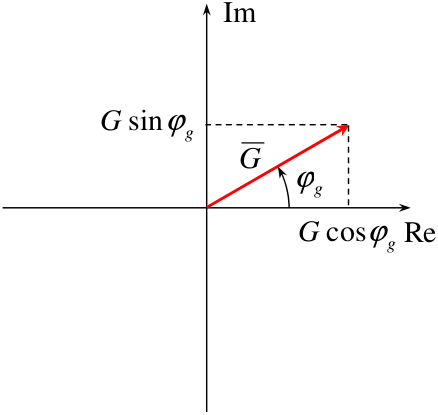
\includegraphics[scale=0.35]{img/dia-phasoriel.png}
	\caption{Diagramme phasoriel.}
	\label{fig:dia-phasoriel}
\end{figure}

On peut retrouver l'expression temporelle d'une grandeur
sinusoïdale en multipliant son phaseur par $e^{j\omega t}$
et en prenant la partie réelle
\begin{equation}
	\Re(\bar{G}e^{j\omega t}) = G\cos(\omega t + \varphi_g) =
	\frac{g}{\sqrt{2}}.
\end{equation}

\subsection{Opérations sur les phaseurs}
On est souvent amené à effectuer des opérations sur les phaseurs,
comme des sommes (en appliquant KCL ou KVL), des
multiplication (pour des calculs de puissances) ou des dérivées
et des intégrales (avec une inductance ou une capacitance).

Lorsqu'on effectue ces opérations il ne faut bien sur pas oublier
qu'un phaseur est un complexe et donc peut être représenté comme
un vecteur. De manière générale, on additionne \textbf{jamais}
simplement des valeurs efficaces : on additionne les phaseurs
correspondants.

\paragraph{Addition}
\begin{align*}
	\bar{G}_\text{tot} 	& = \bar{G}_1 + \bar{G}_2 \\
						&= (G_1\cos \varphi_{g1} + G_2\cos \varphi_{g2})
						+ j(G_1\sin \varphi_{g1} + G_2\cos \varphi_{g2})
\end{align*}

\paragraph{Multiplication}
\begin{align*}
	\bar{G}_\text{tot} 	& = \bar{G}_1 \cdot \bar{G}_2 \\
						&= G_1G_2 e^{j(\varphi_{g1} + \varphi_{g2})}
\end{align*}

\paragraph{Dérivation}
\begin{equation*}
	\fdif{\bar{G}}{t} = j\omega\bar{G} = e^{j\frac{\pi}{2}}\omega
	\bar{G} = \omega G e^{j(\varphi + \frac{\pi}{2})}
\end{equation*}

Pour une inductance dont la relation courant-tension est donnée par
$v = L\fdif{i}{t}$, on retrouve bien que la tension est en avance
de 90° sur le courant.

\paragraph{Intégration}
\begin{equation*}
	\int \bar{G} \dif t = \frac{\bar{G}}{j\omega}
	= e^{-j\frac{\pi}{2}}\frac{\bar{G}}{j\omega}
	= \frac{G}{\omega}e^{j(\varphi-\frac{\pi}{2})}
\end{equation*}

Pour une capacitance dont la relation courant-tension est donnée par
$i = c\fdif{v}{t}$, on retrouve bien que la tension est en retard
de 90° sur le courant.

%TODO convention récepteur/émetteur

\section{Puissances}
Dans cette section, on définit les différentes puissances dans
le cas général et dans le cas particulier de grandeurs
sinusoïdales (égalité indiquée par $\stackrel{\sin}{=}$).

\begin{mydef}[Puissance instantanée]
La puissance instantanée $p$ d'un élément de circuit
est donnée par
\begin{equation}
	p \eqdef ui \stackrel{\sin}{=} <p> + UI\cos(2\omega t +
	\varphi_u + \varphi_i)
	\u{\watt}
	\label{eq:p-inst}
\end{equation}
où $u$ est la tension instantanée aux bornes de cet élément
et $i$ le courant le traversant. On remarque donc que la
puissance instantannée est constituée d'une partie constante
égale à la puissance moyenne et d'une partie oscillante à 2 fois
la fréquence de la tension et du courant.
\end{mydef}

\begin{mydef}[Puissance complexe]
La puissance complexe $\bar{S}$ d'un élément est donnée par
\begin{equation}
	\bar{S} \eqdef \frac{1}{2}\bar{V}\bar{I}^*
	\stackrel{\sin}{=} UIe^{j\varphi}. 
	\u{\volt\ampere}
\end{equation}
On peut décomposer cette puissance complexe en une partie
réelle $P$ qu'on appelle la puissance active et une partie
imaginaire $Q$ qu'on appelle la puissance réactive.
\begin{equation}
	\bar{S} = P + jQ.
\end{equation}
La norme $S$ de $\bar{S}$ est appelée la puissance apparente.
\end{mydef}

\begin{mydef}[Puissance active]
La puissance \textbf{active} $P$ est la moyenne de la
puissance instantanée
\begin{equation}
	P \eqdef\Re(\bar{S}) \stackrel{\sin}{=} \la p \ra = \la ui \ra
	= UI\cos(\varphi).
	\u{\watt}
\end{equation}
Par défaut, lorsqu'on parle de puissance d'une impédance, on
parle de puissance active. Intuitivement, la puissance active
traduit un échange d'énergie unilatéral entre la source et
une charge. En d'autres termes, il s'agit de la puissance
dissipée et perdue à tout jamais (dans une résistance par exemple).
Dans cette dernière équation, on remarque que $P = 0$ si $\varphi =
\pm \frac{\pi}{2}$. C'est à dire si l'élément est purement inductif
ou capacitif. 
\end{mydef}

\begin{mydef}[Puissance réactive]
La puissance \textbf{réactive} $Q$ n'apparaît qu'en présence
d'un élément inductif ou capacitif. Elle traduit un échange bilatéral
d'énergie entre la source et la charge. En d'autres termes, il
s'agit de la puissance stockée et reçue de manière réversible dans
l'impédance.
\begin{equation}
	Q \eqdef \Im(\bar{S}) \stackrel{\sin}{=} UI\sin(\varphi).
	\u{\volt\ampere r}
\end{equation}
Ses unités sont des volts ampères réactifs.
On remarque bien dans cette dernière équation que $Q = 0$ si
$\varphi = 0$, c'est à dire si le courant et la tension sont
parfaitement en phase et donc que l'élément de circuit est purement
résistif. 

On parle d'éléments inductifs lorsqu'ils \og absorbent \fg{} de
la puissance réactive ($Q > 0$), c'est à dire quand
\[ 0 < \varphi \leq \frac{\pi}{2} \]
et d'éléments réactifs lorsqu'ils \og produisent \fg{} de la
puissance réactive ($Q < 0$), c'est à dire quand
\[ -\frac{\pi}{2} \leq \varphi < 0. \]
\end{mydef}

\begin{mydef}[Puissance apparente]
La puissance \textbf{apparente} $S$ est le  produit des
valeurs efficaces de la tension et du courant
\begin{equation}
	S \eqdef |\bar{S}| = \sqrt{P^2 + Q^2} \stackrel{\sin}{=} UI.
	\u{\volt\ampere}
\end{equation}
\end{mydef}

\`{A} partir de toutes ces définitions, on peut réecrire la
puissance instantanée (équation \ref{eq:p-inst}) de grandeurs
sinusoïdales comme
\begin{equation}
	p = P + S\cos(2\omega t + \varphi_u + \varphi_i).
\end{equation}

Le bilan de puissance complexe sur un circuit isolé est toujours
nul
\begin{equation}
	\sum \bar{S} = 0
\end{equation}
et donc
\begin{align}
	\sum P & = 0 & \sum Q & = 0. 
\end{align}

\begin{mydef}[Facteur de puissance]
On définit le facteur de puissance $fp$
\begin{equation}
	fp \eqdef \frac{P}{S} \stackrel{\sin}{=} \cos\varphi.
\end{equation}
\end{mydef}

\section{Impédances}
\subsection{Généralités}
\begin{mydef}
En phasoriel, l'impédance se définit
\begin{equation}
	\bar{Z} \eqdef \frac{\bar{U}}{\bar{I}}.
\end{equation}
Son utilisation n'est valable que dans le cas
\begin{itemize}
	\item d'un régime sinusoïdal établi ;
	\item de composants linéraires.
\end{itemize}
\end{mydef}

On retrouve facilement les impédances des éléments
de circuits habituels.
\begin{align*}
	\bar{Z} & = R 					& \text{pour une résistance,} \\
	\bar{Z} & = j\omega L 			& \text{pour une inductance,} \\
	\bar{Z} & = \frac{1}{j\omega C}	& \text{pour une capacitance.} 
\end{align*}
On remarque que l'impédance est une fonction de la fréquence pour
l'inductance et la capacitance.

\begin{myrem}
Quand l'effet de peau n'est pas négligeable (à haute fréquence), la
résistance dépend également de la fréquence (voir cours
LELEC1350 - électromagnétisme appliqué).
\end{myrem}

On simplifie des impédances en séries et en parallèles de la même
manière que des résistances (en gardant en tête que l'impédance est
un nombre comlexe).

\subsection{Substitutions étoile - triangle}
En régime triphasé on est régulièrement amené à travailler avec des
configurations d'impédances en étoile ou en triangle comme illustré à la
figure \ref{fig:sub-star-triangle}.

\begin{figure*}[ht!]
    \centering
    \begin{subfigure}[t]{0.45\textwidth}
        \centering
        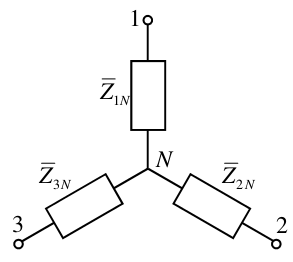
\includegraphics[height=1.2in]{img/star.png}
        \caption{En étoile.}
    \end{subfigure}%
    $\Longrightarrow$
    \begin{subfigure}[t]{0.45\textwidth}
        \centering
        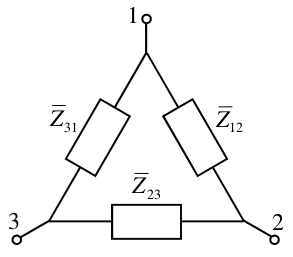
\includegraphics[height=1.2in]{img/triangle.png}
        \caption{En triangle.}
    \end{subfigure}
    \caption{Subsitutions étoile - triangle}
    \label{fig:sub-star-triangle}
\end{figure*}

On peut passer de triangle à étoile en utilisant
\begin{align*}
	\bar{Z}_{1N} &= \frac{\bar{Z}_{31}\bar{Z}_{12}}{\bar{Z}_{12}+\bar{Z}_{23}+\bar{Z}_{31}} &
	\bar{Z}_{2N} &= \frac{\bar{Z}_{12}\bar{Z}_{23}}{\bar{Z}_{12}+\bar{Z}_{23}+\bar{Z}_{31}} &
	\bar{Z}_{3N} &= \frac{\bar{Z}_{23}\bar{Z}_{31}}{\bar{Z}_{12}+\bar{Z}_{23}+\bar{Z}_{31}}
\end{align*}
et d'étoile à triangle en utilisant
\begin{align*}
	\bar{Z}_{31} &= \bar{Z}_{3N} + \bar{Z}_{1N} + \frac{\bar{Z}_{3N}\bar{Z}_{1N}}{\bar{Z_{2N}}} &
	\bar{Z}_{12} &= \bar{Z}_{1N} + \bar{Z}_{2N} + \frac{\bar{Z}_{1N}\bar{Z}_{2N}}{\bar{Z_{3N}}} &
	\bar{Z}_{23} &= \bar{Z}_{2N} + \bar{Z}_{3N} + \frac{\bar{Z}_{2N}\bar{Z}_{3N}}{\bar{Z_{1N}}}.
\end{align*}

Fort heureusement, ces horribles formules se simplifient grandement dans
le cas de configurations équilibrées, c'est à dire quand $\bar{Z}_{1N} =
\bar{Z}_{2N} = \bar{Z}_{3N} = \bar{Z}_N$ et quand $\bar{Z}_{31} = \bar{Z}_{12} =
\bar{Z}_{23} = \bar{Z}$. Dans ce cas, on peut passer de triangle à étoile en utilisant
\begin{equation*}
	\bar{Z}_N = \frac{\bar{Z}}{3}
\end{equation*}
et d'étoile à triangle en utilisant
\begin{equation*}
	\bar{Z} = 3\bar{Z}_N.
\end{equation*}

\section{Mesures en électrotechnique}
\subsection{Généralités}
Les mesures des \textbf{valeurs efficaces} de la tension et du
courant s'effectuent respectivement avec un voltmètre
et un ampèremètre. On peut également mesurer la
\textbf{puissance active} à l'aide d'un wattmètre.

Lorsqu'on effectue des mesures, il faut faire attention
aux erreurs causées par l'insertion d'un appareil de mesure
(voir figure \ref{fig:mes-errors}).

\begin{figure*}[ht!]
    \centering
    \begin{subfigure}[t]{0.5\textwidth}
        \centering
        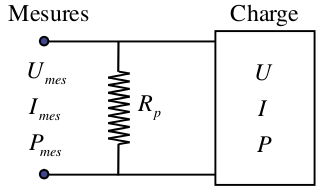
\includegraphics[height=1.2in]{img/mes-insert.png}
        \caption{Dans cet exemple, on souhaite mesurer la tension
        $U$ à l'aide d'un voltmère que l'on connecte donc en parallèle
        avec la charge. La résistance interne du voltmètre $R_p$ est
        donc en parallèle avec la charge et va perturber le
        fonctionnement du circuit. Pour un voltmètre idéal,
        $R_p \to \infty$ et on peut négliger cette perturbation.}
    \end{subfigure}%
    ~
    \begin{subfigure}[t]{0.5\textwidth}
        \centering
        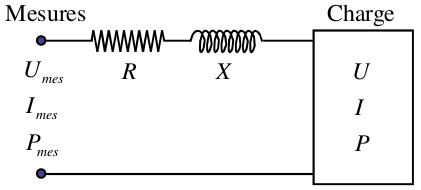
\includegraphics[height=1.2in]{img/mes-bad-link.png}
        \caption{Dans cet exemple, on souhaite mesurer le courant
        $I$ circulant dans la charge à l'aide d'un ampèremètre que l'on
        connecte donc en série avec la charge. L'impédance interne
        du voltmètre, constitué ici d'une résistance $R$ et d'une
        inductance $X$, va perturber le circuit. Pour
        un ampèremètre idéal, $R$ et $X \to 0$ et on peut négligler
        cette pertubation.}
    \end{subfigure}
    \caption{Erreur de mesure due à l'insertion d'un appareil
    de mesure (a) et erreur de mesure due à une liaison non-idéale (b).}
    \label{fig:mes-errors}
\end{figure*}

\subsection{Mesures d'impédances}
Pour mesurer une impédance, c'est à dire un nombre complexe,
il faut effectuer deux mesures
\begin{align*}
	|\bar{Z}| & = Z = \frac{U_\text{mes}}{I_\text{mes}}, \\
	\arg \bar{Z} & = \varphi = \arccos\left(\frac{P_\text{mes}}
	{U_\text{mes}I_\text{mes}}\right).
\end{align*}
% FIX: discussion avec @cassiersg, @bilal1509 et @pverbist sur la formule
% pour l'argument de Z.

On peut ensuite trouver un circuit équivalent série (figure
\ref{fig:eq-circ} (a))
\begin{align*}
	R_s & = Z\cos\varphi & X_s & = \sin\varphi
\end{align*}
et un circuit équivalent parallèle (figure \ref{fig:eq-circ} (b))
\begin{align*}
	R_p & = \frac{Z}{\cos\varphi} & X_p & = \frac{Z}{\sin\varphi}.
\end{align*}

\begin{figure*}[ht!]
    \centering
    \begin{subfigure}[t]{0.5\textwidth}
        \centering
        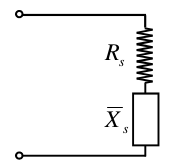
\includegraphics[height=1.2in]{img/eq-circ-series.png}
        \caption{Circuit équivalent série.}
    \end{subfigure}%
    ~
    \begin{subfigure}[t]{0.5\textwidth}
        \centering
        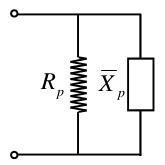
\includegraphics[height=1.2in]{img/eq-circ-para.png}
        \caption{Circuit équivalent parallèle.}
    \end{subfigure}
    \caption{Circuits équivalents d'une impédance.}
    \label{fig:eq-circ}
\end{figure*}

\part{Les transformateurs de puissance}
\section{Le transformateur monophasé}
\subsection{Généralités}
Un transformateur permet d'adapter le niveau d'une tension
\textbf{alternative sinusoïdale}. Il peut fonctionner en
\emph{élévateur} de tension ou en \emph{abaisseur} de tension.

Un transformateur est utile pour
\begin{itemize}
	\item le transport de l'énergie : augmenter la tension permet, à
	puissance transmise donnée, de réduire le courant et donc de réduire
	les pertes de puissance (rappelons que $p = Ri^2$) et/ou de réduire
	la section des conducteurs (ce qui augmente la résistance puisque
	$R = \rho\frac{L}{S}$ mais permet de faire des économies de cuivres) ;
	\item adaptation du niveau de tension pour des applications \og domestiques
	\fg{} : permet par exemple d'obtenir du \SI{12}{\volt} à partir du
	réseau électrique à \SI{230}{\volt} (figure \ref{fig:adapt-dom}).
\end{itemize}

\begin{figure}[ht]
	\centering
	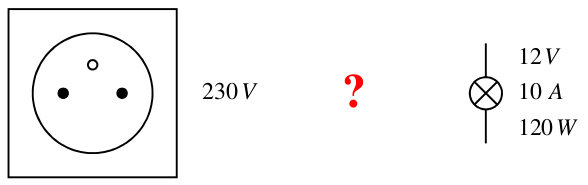
\includegraphics[scale=0.35]{img/adapt-dom.png}
	\caption{Comment adapter le niveau tension à un usage domestique?}
	\label{fig:adapt-dom}
\end{figure}

Dans le cas de la deuxième utilité du transformateur, on pourrait se
poser la question suivante : pourquoi ne pas simplement utiliser un
diviseur d'impédance pour abaisser la tension, comme illustré à la
figure \ref{fig:adapt-dom-bad} ?

\begin{figure}[ht]
	\centering
	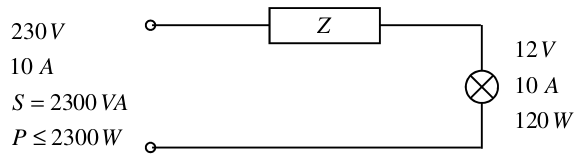
\includegraphics[scale=0.35]{img/adapt-dom-bad.png}
	\caption{Adaptation à l'aide d'un diviseur d'impédance : mauvaise
	solution.}
	\label{fig:adapt-dom-bad}
\end{figure}

La réponse est évidente. En faisant de la sorte, l'impédance $Z$ dissipe
en permanence de l'énergie. On a donc un rendement (puissance utilisée
divisée par la puissance pour laquelle on paye) très mauvais.

En utilisant un transformateur comme illustré sur la figure
\ref{fig:adapt-dom-good}, on garantit un rendement maximal.

\begin{figure}[ht]
	\centering
	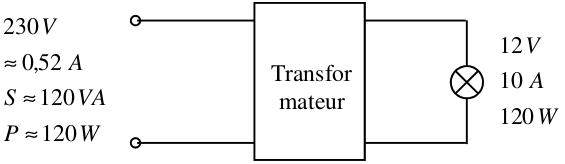
\includegraphics[scale=0.35]{img/adapt-dom-good.png}
	\caption{Adaptation à l'aide d'un transformateur : bonne solution.}
	\label{fig:adapt-dom-good}
\end{figure}

\subsection{Rappels d'électromagnétisme}
Un conducteur parcouru par un courant génère un champ magnétique
$\H$ selon la loi d'Ampère
\[ \oint_\Gamma \H \cdot \dl = Ni. \]
La présence d'un matériau ferromagnétique (c'est à dire un matériau
pour lequel $\mu_r >> 1$) permet de canaliser les lignes de champ.
Un circuit fermé soumis à un flux magnétique $\Phi$ variable
est le siège d'une force électromotrice $\EMF$ selon la loi de Lenz
\[ \EMF = -\fdif{\Phi}{t}. \]
Enfin, rappelons que le flux magnétique est donné par
\[ \Phi = \int_S \B \cdot \dS \]
et que le champ $\B$ est donné par
\[ \B = \mu \H. \]
C'est tout ce dont nous avons besoin pour établir les lois
fondamentales du transformateur.

\subsection{Structure des transformateurs}
\paragraph{En colonne}
Dans une structure en \emph{colonne} comme sur la figure
\ref{fig:struct-colonne}, les spires du primaire et du secondaire
sont enroulées sur deux \og colonnes \fg{} différentes.

\begin{figure}[ht]
	\centering
	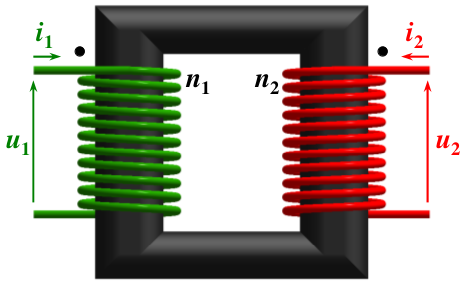
\includegraphics[scale=0.35]{img/struct-colonne.png}
	\caption{Structure en colonne.}
	\label{fig:struct-colonne}
\end{figure}

\paragraph{En manteau}
Dans une structure en \emph{manteau} comme sur la figure
\ref{fig:struct-manteau}, les spires du primaire et du
secondaire sont enroulées sur une même \og colonnes \fg{}.
Cette structure offre une certaine robustesse mécanique
puisque les spires sont protégées par les \og colonne \fg{}
extérieures. Hormis cette différence mécanique, le comportement
électromagnétique est pratiquement le même. 

\begin{figure}[ht]
	\centering
	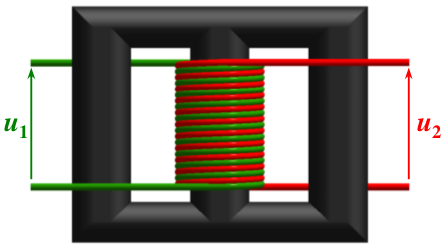
\includegraphics[scale=0.35]{img/struct-manteau.png}
	\caption{Stucture en manteau.}
	\label{fig:struct-manteau}
\end{figure}

\begin{myrem}[Bornes homologues]
Sur la figure \ref{fig:struct-colonne}, on remarque deux points
noirs $\bullet$ sur chaque bobine. Ces symboles indiquent les
bornes homologues du transformateur et permettent de prendre en
compte le sens du bobinage.
\begin{itemize}
	\item Quand le courant entre par la borne homologue, il induit une
	tension positive à la borne homologue de l'autre bobine ;
	\item Quand le courant entre par l'autre borne, il induit une tension
	positive à l'autre borne de l'autre bobine.
\end{itemize}
\end{myrem}

\subsection{Loi fondamentales du transformateur}
\subsubsection{Relation flux - tensions}
\begin{myhyp}
On néglige les fuites magnétiques. On considère donc que le flux est
concentré et conservé le circuit magnétique.
\label{hyp:no-leak}
\end{myhyp}

Sous cette hypothèse, on a
\begin{align*}
	\Psi_1 & = n_1\phi & \text{ au primaire,} \\
	\Psi_2 & = n_2\phi &	 \text{ au secondaire,}
\end{align*}
où $\phi$ est le flux élémentaire circulant dans le circuit
magnétique. Et donc,
\begin{equation*}
	\frac{\Psi_2}{\Psi_1} = \frac{n_2}{n_1}.
\end{equation*}
Or flux et tension sont liés par loi de Faraday
\begin{equation}
	u = \fdif{\Psi}{t} + Ri
	\label{eq:faraday-transfo}
\end{equation}
où $R$ est la résistance des enroulements.

\begin{myhyp}
On néglige la résistance des enroulements : $R = 0$.
\label{hyp:res-nulle}
\end{myhyp}

On obtient donc finalement
\begin{equation}
	\frac{u_1}{u_2} = \frac{n_1}{n_2} \eqdef k.
	\label{eq:transfo-ideal-tension}
\end{equation}

\subsection{Relation champ magnétique - courant}
On applique la loi d'Ampère sur la structure en colonne de la
figure \ref{fig:struct-colonne}, ce qui donne
\[ \oint_\Gamma \H \cdot \dl = n_1i_1 + n_2i_2. \]

\begin{myhyp}
On considère un matériau ferromagnétique parfait, c'est à dire
pour lequel $\mu_r = \infty$. Notons que cette hypothèse est
implicitement incluse dans l'hypothèse \ref{hyp:no-leak}.
\label{hyp:perm-infty}
\end{myhyp}

Comme $\B$ est fixé par $u$ et par la surface des spires qui
sont des quantités finies, $\B$ est également une quantité finie.
Et donc,
\begin{equation*}
	\H = \frac{\B}{\mu_0\mu_r} \to 0.
\end{equation*}

L'application de la loi d'Ampère sur la structure en colonne
devient donc
\begin{equation}
	n_1i_1 + n_2i_2 = 0 \Rightarrow \frac{i_1}{i_2} = -\frac{n_2}{n_1} =
	-\frac{1}{k}.
	\label{eq:transfo-ideal-courant}
\end{equation}

\subsection{Transformateur idéal}
Les équations \ref{eq:transfo-ideal-tension} et \ref{eq:transfo-ideal-courant}
constituent les équations constitutives du transformateur idéal dont
le symbole est donné par la figure \ref{fig:transfo-ideal}.

\begin{figure}[ht!]
	\centering
	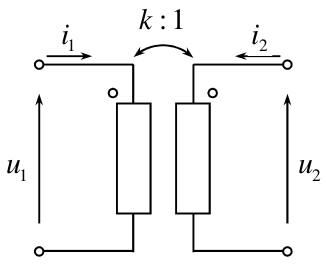
\includegraphics[scale=0.35]{img/transfo-ideal.png}
	\caption{Transformateur idéal. Pour une spire au secondaire,
	on a $k$ spires au primaire.}
	\label{fig:transfo-ideal}
\end{figure}

\subsubsection{Propriétés du transformateur idéal}
\begin{myprop}[Non-énergétique]
Le transformateur idéal est non-énergétique, c'est à dire qu'il ne consomme
et ne produit pas d'énergie. C'est une conséquence directe des équations
constitutives du transformateur idéal
\begin{equation}
	u_1i_1 + u_2i_2 = 0.
\end{equation}
\end{myprop}

\begin{myprop}[Manipulations de circuit aisées]
Comme illustrés aux figures \ref{fig:manip-transfo-ideal-1}
et \ref{fig:manip-transfo-ideal-2}, on peut faire passer une
impédance en série ou en parallèle du primaire au secondaire
et inversement. Pour se convaincre de l'équivalence, on peut
comparer l'énergie dissipée par l'impédance dans le primaire et
dans le secondaire.

\begin{figure}[ht!]
	\centering
	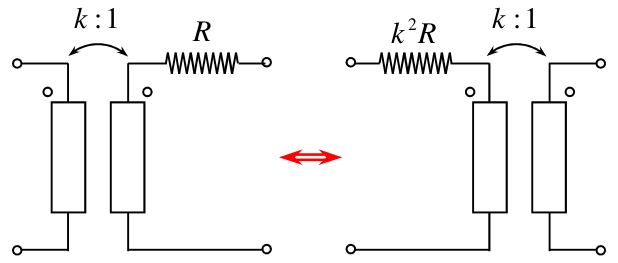
\includegraphics[scale=0.35]{img/manip-transfo-ideal-1.png}
	\caption{Passage de résistance en série du primaire au secondaire
	(et inversement).}
	\label{fig:manip-transfo-ideal-1}
\end{figure}

\begin{figure}[ht!]
	\centering
	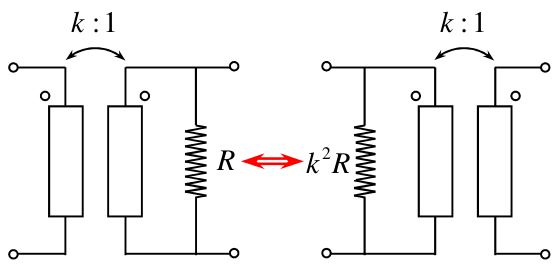
\includegraphics[scale=0.35]{img/manip-transfo-ideal-2.png}
	\caption{Passage de résistance en parallèle du primaire au secondaire
	(et inversement).}
	\label{fig:manip-transfo-ideal-2}
\end{figure}
\end{myprop}

\begin{myexem}[Adaptation d'impédance]
La dernière propriété permet par exemple de faire de l'adaptation
d'impédance. Prenons par exemple un haut-parleur de \SI{4}{\ohm} que
l'on souhaite connecter à un amplificateur de même puissance mais prévu
pour une impédance de charge de \SI{2}{\ohm}. On peut utiliser un
transformateur dont le $k$ a été choisi afin que l'amplificateur voit
une charge de \SI{2}{\ohm}, comme illustré à la figure \ref{fig:adapt-imp}.

\begin{figure}[ht!]
	\centering
	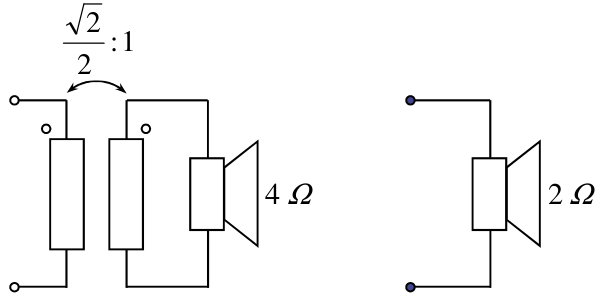
\includegraphics[scale=0.35]{img/adapt-imp.png}
	\caption{Exemple d'adaptation d'impédance à l'aide d'un transformateur.}
	\label{fig:adapt-imp}
\end{figure}
\end{myexem}

\subsection{Le transformateur parfait}
\'{E}cartons-nous maintenant du transformateur idéal en retirant une
par une les hypothèses posées précédemment.

\paragraph{Matériau magnétique parfait} 
On commence par supprimer l'hypothèse \ref{hyp:perm-infty} ; le matériau
ferromagnétique ne possède plus une perméabilité magnétique infinie.
On a donc maintenant $H \neq 0$, et donc l'application de la loi d'Ampère
sur le circuit magnétique nous donne
\[ n_1i_1 + n_2i_2 \neq 0. \]
Du point de vue primaire (on peut faire le même raisonnement à partir
du secondaire), cela signifie que
\[ i_1\big|_{i_2 = 0} = i_{10} \eqdef i_\mu \neq 0. \]
On appelle $i_{10} =  i_\mu$ le courant \emph{à vide} ou le courant
\emph{magnétisant} du transformateur. D'un point de vue circuit, on
modélise ce comportement en ajoutant une impédance parallèle à l'entrée
du primaire, comme illustré à la figure \ref{fig:mod-transfo-parfait-1}.

\begin{figure}[ht!]
	\centering
	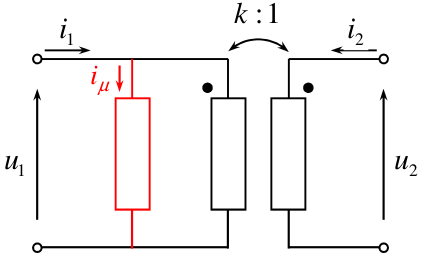
\includegraphics[scale=0.35]{img/mod-transfo-parfait-1.png}
	\caption{Modélisation du courant à vide côté primaire.}
	\label{fig:mod-transfo-parfait-1}
\end{figure}

Essayons maintenant de déterminer cette impédance. Pour cela, on
applique la loi d'Ampère et on calcule le flux élémentaire circulant
dans le circuit magnétique du transformateur à vide (voir figure
\ref{fig:circ-magn-transfo-a-vide}) en prenant 3 hypothèses :
\begin{enumerate}
	\item $H$ est constant le long du circuit magnétique ;
	\item $H$ est constant sur la section du circuit magnétique ;
	\item Le flux est conservé dans le circuit magnétique.
\end{enumerate}

\begin{figure}[ht!]
	\centering
	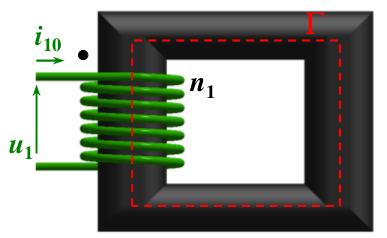
\includegraphics[scale=0.35]{img/circ-magn-imp.png}
	\caption{Circuit magnétique du transformateur à vide.}
	\label{fig:circ-magn-transfo-a-vide}
\end{figure}

On obtient donc
\[ \oint_\Gamma \H \cdot \dl = \Gamma H = n_1i_{10} \]
et
\[ \Phi = \int_S \B \cdot \dS = BS = \mu HS. \]
En combinant les deux, on obtient le flux élémentaire circulant
dans le circuit magnétique.
\[ \Phi = \mu S\frac{n_1i_{10}}{\Gamma}. \]
En se rappellant de la loi d'Hopkinson (analogue à la loi d'Ohm)
\[ \Phi = \frac{\MMF}{\relu} \]
on trouve la force magnétomotrice et la reluctance
\begin{align*}
	\MMF & = n_1i_{10} & \relu & = \frac{\Gamma}{\mu S}.
\end{align*}
Le flux total intercepté par le primaire est simplement donné par
\[ \Psi_1 = n_1\Phi = \mu S\frac{n_1^2i_{10}}{\Gamma}. \]
En utilisant la loi de Faraday (équation \ref{eq:faraday-transfo})
en négligeant toujours la résistance des enroulements on obtient
\begin{equation}
	u_1 = \fdif{\Psi_1}{t} = \frac{\mu S}{\Gamma}n_1^2
	\fdif{i_{10}}{t} = L_\mu\fdif{i_{10}}{t}.
\end{equation}
L'impédance qu'on recherche et donc une inductance, qu'on appelle
\emph{inductance magnétisante} dont la valeur est donnée par
\begin{equation}
	L_\mu = \frac{\mu S}{\Gamma}n_1^2 = n_1^2\frac{1}{\relu}
	= n_1^2\Lambda
\end{equation}
où $\Lambda = 1/\relu$ est la \emph{perméance} du circuit magnétique.
Le modèle de la figure \ref{fig:mod-transfo-parfait-1} se précise et
est donné sur la figure \ref{fig:mod-transfo-parfait-2}.

\begin{figure}[ht!]
	\centering
	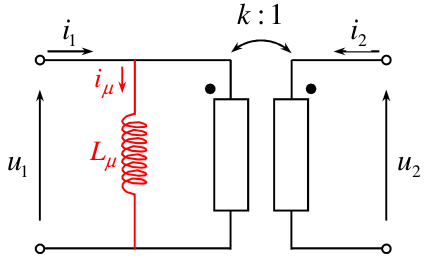
\includegraphics[scale=0.35]{img/mod-transfo-parfait-2.png}
	\caption{Modélisation plus précise du courant à vide côté primaire.}
	\label{fig:mod-transfo-parfait-2}
\end{figure}

\begin{myrem}
On peut faire le même raisonnement du côté du secondaire. Par symétrie,
on obtiendra la même inductance magnétisante avec $n_2$ à la place de
$n_1$. On obtient le même résultat en utilisant les manipulations de
circuit présentées aux figures \ref{fig:manip-transfo-ideal-1} et
\ref{fig:manip-transfo-ideal-2}.
\end{myrem}

\begin{myrem}
On sait donc maintenant que laisser un chargeur d'ordinateur 
(transformateur abaisseur de tension) branché dans
une prise sans que l'ordinateur soit en charge consomme quand même un
courant. Cependant, on voit que ce courant est purement réactif. D'un point
de vue économique ce n'est pas grave car le particulier ne paye pas le
courant réactif.
D'un point de vue écologique c'est beaucoup moins bien car ce courant est
quand même transporté par le réseau et engendre donc des pertes.
\end{myrem}

Malheureusement ce n'est pas encore tout à fait fini car $L_\mu$ est
une fonction de $\mu$ et $\mu$ n'est pas constant.

%TODO : relation constitutive non-linéaire
%TODO : bien définir les différences entre transformateur idéal, parfait et réel

\subsection{Le transformateur réel}
\paragraph{Résistance des enroullements nulles}
On supprime maintenant l'hypothèse \ref{hyp:res-nulle}. Dans ce cas, on ne
peut plus négliger le terme $Ri$ dans l'équation \ref{eq:faraday-transfo}.
On modélise cet effet en ajoutant simplement une résistance série de chaque
cûté du transformateur (figure \ref{fig:mod-res-non-nulles}).

 \begin{figure}[ht!]
	\centering
	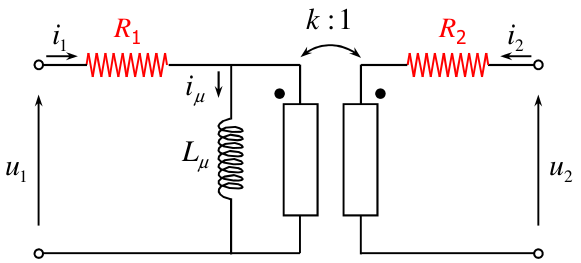
\includegraphics[scale=0.35]{img/mod-res-non-nulles.png}
	\caption{Modélisation de la résistance des enroullements.}
	\label{fig:mod-res-non-nulles}
\end{figure}

\section{Le transformateur triphasé}

\part{Les convertisseurs électromécaniques}
\section{Introduction générale}
\section{Théorie générale}
\section{Les machines à champ tournant}
\section{La machine asynchrone}
\section{La machine synchrone}
\section{La machine à courant continu}

\end{document}
